\columnratio{0.55}
\begin{paracol}{2}
\switchcolumn[0]*%%%%%%%
\section{Slots}
\switchcolumn
\section{插槽 Slots}
\switchcolumn[0]*%%%%%%%
\begin{quote}
This page assumes you've already read the
\href{https://vuejs.org/guide/essentials/component-basics.html}{Components
Basics}. Read that first if you are new to components.
\end{quote}
\switchcolumn
\begin{quote}
此章节假设你已经看过了\href{https://cn.vuejs.org/guide/essentials/component-basics.html}{组件基础}。若你还不了解组件是什么,请先阅读该章节。
\end{quote}
\switchcolumn[0]*%%%%%%%
\subsection{Slot Content and Outlet}
\switchcolumn
\subsection{插槽内容与出口}
\switchcolumn[0]*%%%%%%%
We have learned that components can accept props, which can be
JavaScript values of any type. But how about template content? In some
cases, we may want to pass a template fragment to a child component, and
let the child component render the fragment within its own template.
\switchcolumn
在之前的章节中,我们已经了解到组件能够接收任意类型的 JavaScript 值作为
props,但组件要如何接收模板内容呢?在某些场景中,我们可能想要为子组件传递一些模板片段,让子组件在它们的组件中渲染这些片段。
\switchcolumn[0]*%%%%%%%
For example, we may have a \texttt{\textless{}FancyButton\textgreater{}}
component that supports usage like this:
\switchcolumn
举例来说,这里有一个 \texttt{\textless{}FancyButton\textgreater{}}
组件,可以像这样使用:
\switchcolumn[0]*%%%%%%%
\begin{codeHtml}
<FancyButton>
  Click me! <!-- 插槽内容 -->
</FancyButton>
\end{codeHtml}
\switchcolumn
\begin{codeHtml}
<FancyButton>
  Click me! <!-- 插槽内容 -->
</FancyButton>
\end{codeHtml}
\switchcolumn[0]*%%%%%%%
The template of \texttt{\textless{}FancyButton\textgreater{}} looks like
this:
\switchcolumn
而 \texttt{\textless{}FancyButton\textgreater{}} 的模板是这样的:
\switchcolumn[0]*%%%%%%%
\begin{codeHtml}
<button class="fancy-btn">
  <slot></slot> <!-- 插槽出口 -->
</button>
\end{codeHtml}
\switchcolumn
\begin{codeHtml}
<button class="fancy-btn">
  <slot></slot> <!-- 插槽出口 -->
</button>
\end{codeHtml}
\switchcolumn[0]*%%%%%%%
The \texttt{\textless{}slot\textgreater{}} element is a \textbf{slot
outlet} that indicates where the parent-provided \textbf{slot content}
should be rendered.
\switchcolumn
\texttt{\textless{}slot\textgreater{}} 元素是一个\textbf{插槽出口} (slot
outlet),标示了父元素提供的\textbf{插槽内容} (slot content)
将在哪里被渲染。
\end{paracol}
\begin{center} 
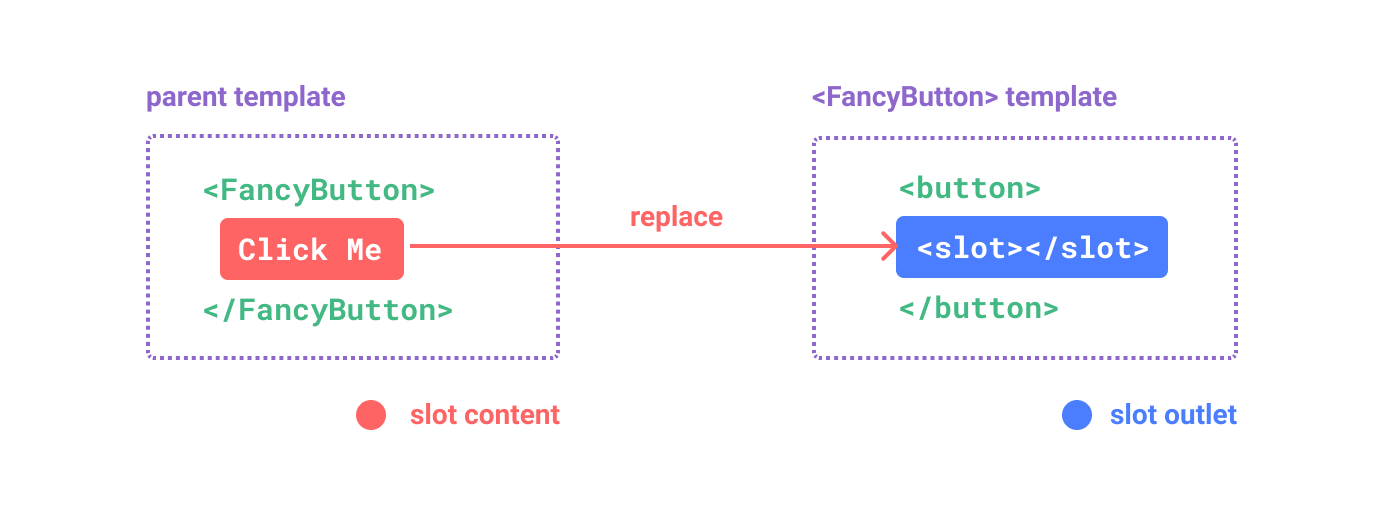
\includegraphics{./img/slots.dbdaf1e8.png} 
\end{center}


\columnratio{0.55}
\begin{paracol}{2}
\switchcolumn[0]*%%%%%%%
And the final rendered DOM:
\switchcolumn
最终渲染出的 DOM 是这样:
\switchcolumn[0]*%%%%%%%
\begin{codeHtml}
<button class="fancy-btn">Click me!</button>
\end{codeHtml}
\switchcolumn
\begin{codeHtml}
<button class="fancy-btn">Click me!</button>
\end{codeHtml}
\switchcolumn[0]*%%%%%%%
\href{https://play.vuejs.org/\#eNpdUdlqAyEU/ZVbQ0kLMdNsXabTQFvoV8yLcRkkjopLSQj596oTwqRvnuM9y9UT+rR2/hs5qlHjqZM2gOch2m2rZW+NC/BDND1+xRCMBuFMD9N5NeKyeNrqphrUSZdA4L1VJPCEAJrRdCEAvpWke+g5NHcYg1cmADU6cB0A4zzThmYckqimupqiGfpXILe/zdwNhaki3n+0SOR5vAu6ReU++efUajtqYGJQ/FIg5w8Wt9FlOx+OKh/nV1c4ZVNqlHE1TIQQ7xnvCN13zkTNalBSc+Jw5wiTac2H1WLDeDeDyXrJVm9LWG7uE3hev3AhHge1cYwnO200L4QljEnd1bCxB1g82UNhe+I6qQs5kuGcE30NrxeaRudzOWtkemeXuHP5tLIKOv8BN+mw3w==}{Try
it in the Playground}
\switchcolumn
\href{https://play.vuejs.org/\#eNpdUdlqAyEU/ZVbQ0kLMdNsXabTQFvoV8yLcRkkjopLSQj596oTwqRvnuM9y9UT+rR2/hs5qlHjqZM2gOch2m2rZW+NC/BDND1+xRCMBuFMD9N5NeKyeNrqphrUSZdA4L1VJPCEAJrRdCEAvpWke+g5NHcYg1cmADU6cB0A4zzThmYckqimupqiGfpXILe/zdwNhaki3n+0SOR5vAu6ReU++efUajtqYGJQ/FIg5w8Wt9FlOx+OKh/nV1c4ZVNqlHE1TIQQ7xnvCN13zkTNalBSc+Jw5wiTac2H1WLDeDeDyXrJVm9LWG7uE3hev3AhHge1cYwnO200L4QljEnd1bCxB1g82UNhe+I6qQs5kuGcE30NrxeaRudzOWtkemeXuHP5tLIKOv8BN+mw3w==}{在演练场中尝试一下}

\switchcolumn[0]*%%%%%%%
With slots, the \texttt{\textless{}FancyButton\textgreater{}} is
responsible for rendering the outer
\texttt{\textless{}button\textgreater{}} (and its fancy styling), while
the inner content is provided by the parent component.
\switchcolumn
通过使用插槽,\texttt{\textless{}FancyButton\textgreater{}}
仅负责渲染外层的 \texttt{\textless{}button\textgreater{}}
(以及相应的样式),而其内部的内容由父组件提供。
\switchcolumn[0]*%%%%%%%
Another way to understand slots is by comparing them to JavaScript
functions:
\switchcolumn
理解插槽的另一种方式是和下面的 JavaScript 函数作类比,其概念是类似的:
\switchcolumn[0]*%%%%%%%
\begin{codeJs}
// 父元素传入插槽内容
FancyButton('Click me!')
// FancyButton 在自己的模板中渲染插槽内容
function FancyButton(slotContent) {
  return `<button class="fancy-btn">
      ${slotContent}
    </button>`
}
\end{codeJs}
\switchcolumn
\begin{codeJs}
// 父元素传入插槽内容
FancyButton('Click me!')
// FancyButton 在自己的模板中渲染插槽内容
function FancyButton(slotContent) {
  return `<button class="fancy-btn">
      ${slotContent}
    </button>`
}
\end{codeJs}
\switchcolumn[0]*%%%%%%%
Slot content is not just limited to text. It can be any valid template
content. For example, we can pass in multiple elements, or even other
components:
\switchcolumn
插槽内容可以是任意合法的模板内容,不局限于文本。例如我们可以传入多个元素,甚至是组件:
\switchcolumn[0]*%%%%%%%
\begin{codeHtml}
<FancyButton>
  <span style="color:red">Click me!</span>
  <AwesomeIcon name="plus" />
</FancyButton>
\end{codeHtml}
\switchcolumn
\begin{codeHtml}
<FancyButton>
  <span style="color:red">Click me!</span>
  <AwesomeIcon name="plus" />
</FancyButton>
\end{codeHtml}
\switchcolumn[0]*%%%%%%%
\href{https://play.vuejs.org/\#eNp1UmtOwkAQvspQYtCEgrx81EqCJibeoX+W7bRZaHc3+1AI4QyewH8ewvN4Aa/gbgtNIfFf5+vMfI/ZXbCQcvBmMYiCWFPFpAGNxsp5wlkphTLwQjjdPlljBIdMiRJ6g2EL88O9pnnxjlqU+EpbzS3s0BwPaypH4gqDpSyIQVcBxK3VFQDwXDC6hhJdlZi4zf3fRKwl4aDNtsDHJKCiECqiW8KTYH5c1gEnwnUdJ9rCh/XeM6Z42AgN+sFZAj6+Ux/LOjFaEK2diMz3h0vjNfj/zokuhPFU3lTdfcpShVOZcJ+DZgHs/HxtCrpZlj34eknoOlfC8jSCgnEkKswVSRlyczkZzVLM+9CdjtPJ/RjGswtX3ExvMcuu6mmhUnTruOBYAZKkKeN5BDO5gdG13FRoSVTOeAW2xkLPY3UEdweYWqW9OCkYN6gctq9uXllx2Z09CJ9dJwzBascI7nBYihWDldUGMqEgdTVIq6TQqCEMfUpNSD+fX7/fH+3b7P8AdGP6wA==}{Try
it in the Playground}
\switchcolumn
\href{https://play.vuejs.org/\#eNp1UmtOwkAQvspQYtCEgrx81EqCJibeoX+W7bRZaHc3+1AI4QyewH8ewvN4Aa/gbgtNIfFf5+vMfI/ZXbCQcvBmMYiCWFPFpAGNxsp5wlkphTLwQjjdPlljBIdMiRJ6g2EL88O9pnnxjlqU+EpbzS3s0BwPaypH4gqDpSyIQVcBxK3VFQDwXDC6hhJdlZi4zf3fRKwl4aDNtsDHJKCiECqiW8KTYH5c1gEnwnUdJ9rCh/XeM6Z42AgN+sFZAj6+Ux/LOjFaEK2diMz3h0vjNfj/zokuhPFU3lTdfcpShVOZcJ+DZgHs/HxtCrpZlj34eknoOlfC8jSCgnEkKswVSRlyczkZzVLM+9CdjtPJ/RjGswtX3ExvMcuu6mmhUnTruOBYAZKkKeN5BDO5gdG13FRoSVTOeAW2xkLPY3UEdweYWqW9OCkYN6gctq9uXllx2Z09CJ9dJwzBascI7nBYihWDldUGMqEgdTVIq6TQqCEMfUpNSD+fX7/fH+3b7P8AdGP6wA==}{在演练场中尝试一下}
\switchcolumn[0]*%%%%%%%
By using slots, our \texttt{\textless{}FancyButton\textgreater{}} is
more flexible and reusable. We can now use it in different places with
different inner content, but all with the same fancy styling.
\switchcolumn
通过使用插槽,\texttt{\textless{}FancyButton\textgreater{}}
组件更加灵活和具有可复用性。现在组件可以用在不同的地方渲染各异的内容,但同时还保证都具有相同的样式。
\switchcolumn[0]*%%%%%%%
Vue components' slot mechanism is inspired by the
\href{https://developer.mozilla.org/en-US/docs/Web/HTML/Element/slot}{native
Web Component {\tt <slot>} element}, but with additional capabilities that we will
see later.
\switchcolumn
Vue
组件的插槽机制是受\href{https://developer.mozilla.org/en-US/docs/Web/HTML/Element/slot}{原生
Web Component {\tt <slot>}
元素}的启发而诞生,同时还做了一些功能拓展,这些拓展的功能我们后面会学习到。
\end{paracol}


\columnratio{0.55}
\begin{paracol}{2}
\switchcolumn[0]*%%%%%%%
\subsection{Render Scope}
\switchcolumn
\subsection{渲染作用域}
\switchcolumn[0]*%%%%%%%
Slot content has access to the data scope of the parent component,
because it is defined in the parent. For example:
\switchcolumn
插槽内容可以访问到父组件的数据作用域,因为插槽内容本身是在父组件模板中定义的。举例来说:
\switchcolumn[0]*%%%%%%%
\begin{codeHtml}
<span>{{ message }}</span>
<FancyButton>{{ message }}</FancyButton>
\end{codeHtml}
\switchcolumn
\begin{codeHtml}
<span>{{ message }}</span>
<FancyButton>{{ message }}</FancyButton>
\end{codeHtml}
\switchcolumn[0]*%%%%%%%
Here both \texttt{\{\{\ message\ \}\}} interpolations will render the
same content.
\switchcolumn
这里的两个 \texttt{\{\{\ message\ \}\}} 插值表达式渲染的内容都是一样的。
\switchcolumn[0]*%%%%%%%
Slot content does \textbf{not} have access to the child component's
data. Expressions in Vue templates can only access the scope it is
defined in, consistent with JavaScript's lexical scoping. In other
words:
\switchcolumn
插槽内容\textbf{无法访问}子组件的数据。Vue
模板中的表达式只能访问其定义时所处的作用域,这和 JavaScript
的词法作用域规则是一致的。换言之:
\switchcolumn[0]*%%%%%%%
\begin{quote}
Expressions in the parent template only have access to the parent scope;
expressions in the child template only have access to the child scope.
\end{quote}
\switchcolumn
\begin{quote}
父组件模板中的表达式只能访问父组件的作用域;子组件模板中的表达式只能访问子组件的作用域。
\end{quote}
\end{paracol}


\columnratio{0.55}
\begin{paracol}{2}

\switchcolumn[0]*%%%%%%%
\subsection{Fallback Content}
\switchcolumn
\subsection{默认内容}
\switchcolumn[0]*%%%%%%%
There are cases when it's useful to specify fallback (i.e. default)
content for a slot, to be rendered only when no content is provided. For
example, in a \texttt{\textless{}SubmitButton\textgreater{}} component:
\switchcolumn
在外部没有提供任何内容的情况下,可以为插槽指定默认内容。比如有这样一个
\texttt{\textless{}SubmitButton\textgreater{}} 组件:
\switchcolumn[0]*%%%%%%%
\begin{codeHtml}
<button type="submit">
    <slot></slot>
</button>
\end{codeHtml}
\switchcolumn
\begin{codeHtml}
<button type="submit">
    <slot></slot>
</button>
\end{codeHtml}
\switchcolumn[0]*%%%%%%%
We might want the text "Submit" to be rendered inside the
\texttt{\textless{}button\textgreater{}} if the parent didn't provide
any slot content. To make "Submit" the fallback content, we can place it
in between the \texttt{\textless{}slot\textgreater{}} tags:
\switchcolumn
如果我们想在父组件没有提供任何插槽内容时在
\texttt{\textless{}button\textgreater{}}
内渲染``Submit'',只需要将``Submit''写在
\texttt{\textless{}slot\textgreater{}} 标签之间来作为默认内容:
\switchcolumn[0]*%%%%%%%
\begin{codeHtml}
<button type="submit">
    <slot>
    Submit <!-- 默认内容 -->
    </slot>
</button>
\end{codeHtml}
\switchcolumn
\begin{codeHtml}
<button type="submit">
    <slot>
    Submit <!-- 默认内容 -->
    </slot>
</button>
\end{codeHtml}
\switchcolumn[0]*%%%%%%%
Now when we use \texttt{\textless{}SubmitButton\textgreater{}} in a
parent component, providing no content for the slot:
\switchcolumn
现在,当我们在父组件中使用
\texttt{\textless{}SubmitButton\textgreater{}}
且没有提供任何插槽内容时:
\switchcolumn[0]*%%%%%%%
\begin{codeHtml}
<SubmitButton />
\end{codeHtml}
\switchcolumn
\begin{codeHtml}
<SubmitButton />
\end{codeHtml}
\switchcolumn[0]*%%%%%%%
This will render the fallback content, "Submit":
\switchcolumn
``Submit''将会被作为默认内容渲染:
\switchcolumn[0]*%%%%%%%
\begin{codeHtml}
<button type="submit">Submit</button>
\end{codeHtml}
\switchcolumn
\begin{codeHtml}
<button type="submit">Submit</button>
\end{codeHtml}
\switchcolumn[0]*%%%%%%%
But if we provide content:
\switchcolumn
但如果我们提供了插槽内容:
\switchcolumn[0]*%%%%%%%
\begin{codeHtml}
<SubmitButton>Save</SubmitButton>
\end{codeHtml}
\switchcolumn
\begin{codeHtml}
<SubmitButton>Save</SubmitButton>
\end{codeHtml}
\switchcolumn[0]*%%%%%%%
Then the provided content will be rendered instead:
\switchcolumn
那么被显式提供的内容会取代默认内容:
\switchcolumn[0]*%%%%%%%
\begin{codeHtml}
<button type="submit">Save</button>
\end{codeHtml}
\switchcolumn
\begin{codeHtml}
<button type="submit">Save</button>
\end{codeHtml}
\switchcolumn[0]*%%%%%%%
\href{https://play.vuejs.org/\#eNp1kMsKwjAQRX9lzMaNbfcSC/oL3WbT1ikU8yKZFEX8d5MGgi2YVeZxZ86dN7taWy8B2ZlxP7rZEnikYFuhZ2WNI+jCoGa6BSKjYXJGwbFufpNJfhSaN1kflTEgVFb2hDEC4IeqguARpl7KoR8fQPgkqKpc3Wxo1lxRWWeW+Y4wBk9x9V9d2/UL8g1XbOJN4WAntodOnrecQ2agl8WLYH7tFyw5olj10iR3EJ+gPCxDFluj0YS6EAqKR8mi9M3Td1ifLxWShcU=}{Try
it in the Playground}
\switchcolumn
\href{https://play.vuejs.org/\#eNp1kMsKwjAQRX9lzMaNbfcSC/oL3WbT1ikU8yKZFEX8d5MGgi2YVeZxZ86dN7taWy8B2ZlxP7rZEnikYFuhZ2WNI+jCoGa6BSKjYXJGwbFufpNJfhSaN1kflTEgVFb2hDEC4IeqguARpl7KoR8fQPgkqKpc3Wxo1lxRWWeW+Y4wBk9x9V9d2/UL8g1XbOJN4WAntodOnrecQ2agl8WLYH7tFyw5olj10iR3EJ+gPCxDFluj0YS6EAqKR8mi9M3Td1ifLxWShcU=}{在演练场中尝试一下}
\end{paracol}

\columnratio{0.55}
\begin{paracol}{2}

\switchcolumn[0]*%%%%%%%
\subsection{Named Slots}
\switchcolumn
\subsection{具名插槽}
\switchcolumn[0]*%%%%%%%
There are times when it's useful to have multiple slot outlets in a
single component. For example, in a
\texttt{\textless{}BaseLayout\textgreater{}} component with the
following template:
\switchcolumn
有时在一个组件中包含多个插槽出口是很有用的。举例来说,在一个
\texttt{\textless{}BaseLayout\textgreater{}} 组件中,有如下模板:
\switchcolumn[0]*%%%%%%%
\begin{codeHtml}
<div class="container">
    <header>
    <!-- 标题内容放这里 -->
    </header>
    <main>
    <!-- 主要内容放这里 -->
    </main>
    <footer>
    <!-- 底部内容放这里 -->
    </footer>
</div>
\end{codeHtml}
\switchcolumn
\begin{codeHtml}
<div class="container">
    <header>
    <!-- 标题内容放这里 -->
    </header>
    <main>
    <!-- 主要内容放这里 -->
    </main>
    <footer>
    <!-- 底部内容放这里 -->
    </footer>
</div>
\end{codeHtml}
\switchcolumn[0]*%%%%%%%
For these cases, the \texttt{\textless{}slot\textgreater{}} element has
a special attribute, \texttt{name}, which can be used to assign a unique
ID to different slots so you can determine where content should be
rendered:
\switchcolumn
对于这种场景,\texttt{\textless{}slot\textgreater{}}
元素可以有一个特殊的 attribute \texttt{name},用来给各个插槽分配唯一的
ID,以确定每一处要渲染的内容:
\switchcolumn[0]*%%%%%%%
\begin{codeHtml}
<div class="container">
    <header>
    <slot name="header"></slot>
    </header>
    <main>
    <slot></slot>
    </main>
    <footer>
    <slot name="footer"></slot>
    </footer>
</div>
\end{codeHtml}
\switchcolumn
\begin{codeHtml}
<div class="container">
    <header>
    <slot name="header"></slot>
    </header>
    <main>
    <slot></slot>
    </main>
    <footer>
    <slot name="footer"></slot>
    </footer>
</div>
\end{codeHtml}
\switchcolumn[0]*%%%%%%%
A \texttt{\textless{}slot\textgreater{}} outlet without \texttt{name}
implicitly has the name "default".
\switchcolumn
这类带 \texttt{name} 的插槽被称为具名插槽 (named slots)。没有提供
\texttt{name} 的 \texttt{\textless{}slot\textgreater{}}
出口会隐式地命名为``default''。
\switchcolumn[0]*%%%%%%%
In a parent component using
\texttt{\textless{}BaseLayout\textgreater{}}, we need a way to pass
multiple slot content fragments, each targeting a different slot outlet.
This is where \textbf{named slots} come in.
\switchcolumn
在父组件中使用 \texttt{\textless{}BaseLayout\textgreater{}}
时,我们需要一种方式将多个插槽内容传入到各自目标插槽的出口。此时就需要用到\textbf{具名插槽}了:
\switchcolumn[0]*%%%%%%%
To pass a named slot, we need to use a
\texttt{\textless{}template\textgreater{}} element with the
\texttt{v-slot} directive, and then pass the name of the slot as an
argument to \texttt{v-slot}:
\switchcolumn
要为具名插槽传入内容,我们需要使用一个含 \texttt{v-slot} 指令的
\texttt{\textless{}template\textgreater{}}
元素,并将目标插槽的名字传给该指令:
\switchcolumn[0]*%%%%%%%
\begin{codeHtml}
<BaseLayout>
  <template v-slot:header>
    <!-- header 插槽的内容放这里 -->
  </template>
</BaseLayout>
\end{codeHtml}
\switchcolumn
\begin{codeHtml}
<BaseLayout>
  <template v-slot:header>
    <!-- header 插槽的内容放这里 -->
  </template>
</BaseLayout>
\end{codeHtml}
\switchcolumn[0]*%%%%%%%
\texttt{v-slot} has a dedicated shorthand \texttt{\#}, so
\texttt{\textless{}template\ v-slot:header\textgreater{}} can be
shortened to just \texttt{\textless{}template\ \#header\textgreater{}}.
Think of it as "render this template fragment in the child component's
'header' slot".
\switchcolumn
\texttt{v-slot} 有对应的简写 \texttt{\#},因此
\texttt{\textless{}template\ v-slot:header\textgreater{}} 可以简写为
\texttt{\textless{}template\ \#header\textgreater{}}。其意思就是``将这部分模板片段传入子组件的
header 插槽中''。
\end{paracol}

\begin{center} 
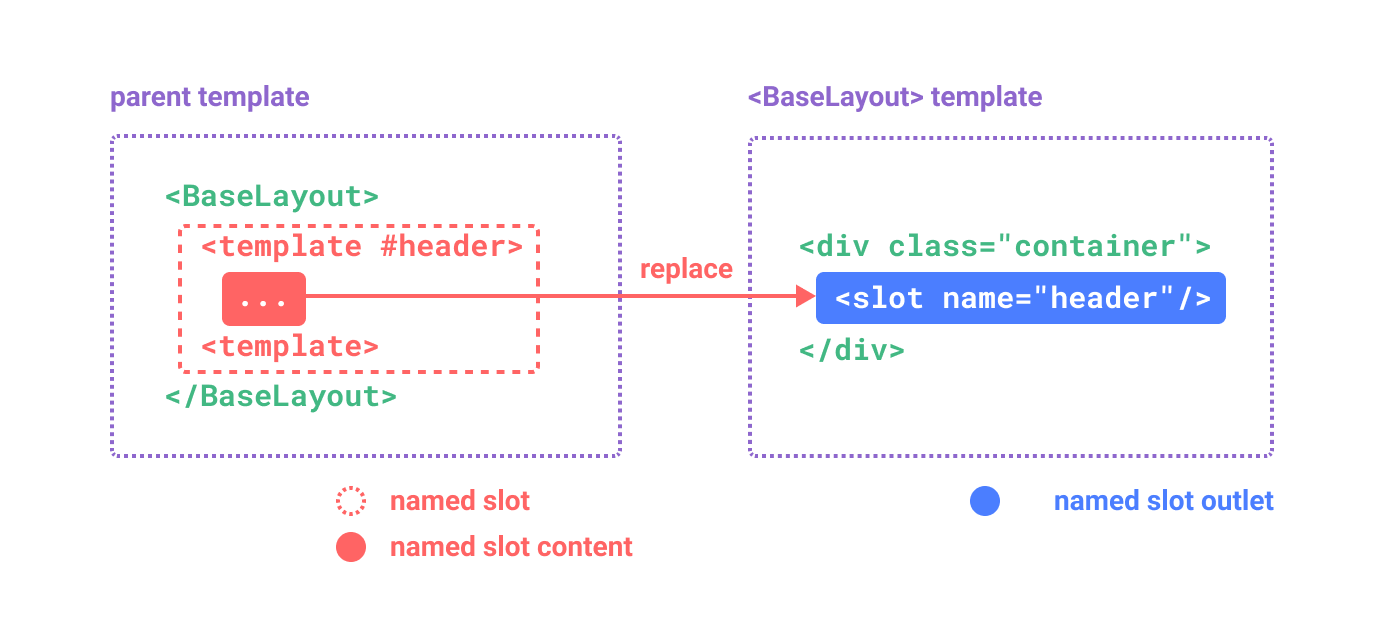
\includegraphics{./img/named-slots.ebb7b207.png} 
\end{center}


\columnratio{0.55}
\begin{paracol}{2}

\switchcolumn[0]*%%%%%%%
Here's the code passing content for all three slots to
\texttt{\textless{}BaseLayout\textgreater{}} using the shorthand syntax:
\switchcolumn
下面我们给出完整的、向 \texttt{\textless{}BaseLayout\textgreater{}}
传递插槽内容的代码,指令均使用的是缩写形式:
\switchcolumn[0]*%%%%%%%
\begin{codeHtml}
<BaseLayout>
    <template #header>
    <h1>Here might be a page title</h1>
    </template>
    <template #default>
    <p>A paragraph for the main content.</p>
    <p>And another one.</p>
    </template>
    <template #footer>
    <p>Here's some contact info</p>
    </template>
</BaseLayout>
\end{codeHtml}
\switchcolumn
\begin{codeHtml}
<BaseLayout>
    <template #header>
    <h1>Here might be a page title</h1>
    </template>
    <template #default>
    <p>A paragraph for the main content.</p>
    <p>And another one.</p>
    </template>
    <template #footer>
    <p>Here's some contact info</p>
    </template>
</BaseLayout>
\end{codeHtml}
\switchcolumn[0]*%%%%%%%
When a component accepts both a default slot and named slots, all
top-level non-\texttt{\textless{}template\textgreater{}} nodes are
implicitly treated as content for the default slot. So the above can
also be written as:
\switchcolumn
当一个组件同时接收默认插槽和具名插槽时,所有位于顶级的非
\texttt{\textless{}template\textgreater{}}
节点都被隐式地视为默认插槽的内容。所以上面也可以写成:
\switchcolumn[0]*%%%%%%%
\begin{codeHtml}
<BaseLayout>
  <template #header>
    <h1>Here might be a page title</h1>
  </template>
  <!-- 隐式的默认插槽 -->
  <p>A paragraph for the main content.</p>
  <p>And another one.</p>
  <template #footer>
    <p>Here's some contact info</p>
  </template>
</BaseLayout>
\end{codeHtml}
\switchcolumn
\begin{codeHtml}
<BaseLayout>
  <template #header>
    <h1>Here might be a page title</h1>
  </template>
  <!-- 隐式的默认插槽 -->
  <p>A paragraph for the main content.</p>
  <p>And another one.</p>
  <template #footer>
    <p>Here's some contact info</p>
  </template>
</BaseLayout>
\end{codeHtml}
\switchcolumn[0]*%%%%%%%
Now everything inside the \texttt{\textless{}template\textgreater{}}
elements will be passed to the corresponding slots. The final rendered
HTML will be:
\switchcolumn
现在 \texttt{\textless{}template\textgreater{}}
元素中的所有内容都将被传递到相应的插槽。最终渲染出的 HTML 如下:
\switchcolumn[0]*%%%%%%%
\begin{codeHtml}
<div class="container">
  <header>
    <h1>Here might be a page title</h1>
  </header>
  <main>
    <p>A paragraph for the main content.</p>
    <p>And another one.</p>
  </main>
  <footer>
    <p>Here's some contact info</p>
  </footer>
</div>
\end{codeHtml}
\switchcolumn
\begin{codeHtml}
<div class="container">
  <header>
    <h1>Here might be a page title</h1>
  </header>
  <main>
    <p>A paragraph for the main content.</p>
    <p>And another one.</p>
  </main>
  <footer>
    <p>Here's some contact info</p>
  </footer>
</div>
\end{codeHtml}
\switchcolumn[0]*%%%%%%%
\href{https://play.vuejs.org/\#eNp9UsFuwjAM/RWrHLgMOi5o6jIkdtphn9BLSF0aKU2ixEVjiH+fm8JoQdvRfu/5xS8+ZVvvl4cOsyITUQXtCSJS5zel1a13geBdRvyUR9cR1MG1MF/mt1YvnZdW5IOWVVwQtt5IQq4AxI2cau5ccZg1KCsMlz4jzWrzgQGh1fuGYIcgwcs9AmkyKHKGLyPykcfD1Apr2ZmrHUN+s+U5Qe6D9A3ULgA1bCK1BeUsoaWlyPuVb3xbgbSOaQGcxRH8v3XtHI0X8mmfeYToWkxmUhFoW7s/JvblJLERmj1l0+T7T5tqK30AZWSMb2WW3LTFUGZXp/u8o3EEVrbI9AFjLn8mt38fN9GIPrSp/p4/Yoj7OMZ+A/boN9KInPeZZpAOLNLRDAsPZDgN4p0L/NQFOV/Ayn9x6EZXMFNKvQ4E5YwLBczW6/WlU3NIi6i/sYDn5Qu2qX1OF51MsvMPkrIEHg==}{Try
it in the Playground}
\switchcolumn
\href{https://play.vuejs.org/\#eNp9UsFuwjAM/RWrHLgMOi5o6jIkdtphn9BLSF0aKU2ixEVjiH+fm8JoQdvRfu/5xS8+ZVvvl4cOsyITUQXtCSJS5zel1a13geBdRvyUR9cR1MG1MF/mt1YvnZdW5IOWVVwQtt5IQq4AxI2cau5ccZg1KCsMlz4jzWrzgQGh1fuGYIcgwcs9AmkyKHKGLyPykcfD1Apr2ZmrHUN+s+U5Qe6D9A3ULgA1bCK1BeUsoaWlyPuVb3xbgbSOaQGcxRH8v3XtHI0X8mmfeYToWkxmUhFoW7s/JvblJLERmj1l0+T7T5tqK30AZWSMb2WW3LTFUGZXp/u8o3EEVrbI9AFjLn8mt38fN9GIPrSp/p4/Yoj7OMZ+A/boN9KInPeZZpAOLNLRDAsPZDgN4p0L/NQFOV/Ayn9x6EZXMFNKvQ4E5YwLBczW6/WlU3NIi6i/sYDn5Qu2qX1OF51MsvMPkrIEHg==}{在演练场中尝试一下}
\switchcolumn[0]*%%%%%%%
Again, it may help you understand named slots better using the
JavaScript function analogy:
\switchcolumn
使用 JavaScript 函数来类比可能更有助于你来理解具名插槽:
\switchcolumn[0]*%%%%%%%
\begin{codeJs}
// 传入不同的内容给不同名字的插槽
BaseLayout({
  header: `...`,
  default: `...`,
  footer: `...`
})
// <BaseLayout> 渲染插槽内容到对应位置
function BaseLayout(slots) {
  return `<div class="container">
      <header>${slots.header}</header>
      <main>${slots.default}</main>
      <footer>${slots.footer}</footer>
    </div>`
}
\end{codeJs}
\switchcolumn
\begin{codeJs}
// 传入不同的内容给不同名字的插槽
BaseLayout({
  header: `...`,
  default: `...`,
  footer: `...`
})
// <BaseLayout> 渲染插槽内容到对应位置
function BaseLayout(slots) {
  return `<div class="container">
      <header>${slots.header}</header>
      <main>${slots.default}</main>
      <footer>${slots.footer}</footer>
    </div>`
}
\end{codeJs}
\end{paracol}


\columnratio{0.55}
\begin{paracol}{2}
 
\switchcolumn[0]*%%%%%%%
\subsection{Dynamic Slot Names}
\switchcolumn
\subsection{动态插槽名}
\switchcolumn[0]*%%%%%%%
\href{https://vuejs.org/guide/essentials/template-syntax.html\#dynamic-arguments}{Dynamic
directive arguments} also work on \texttt{v-slot}, allowing the
definition of dynamic slot names:
\switchcolumn
\href{https://cn.vuejs.org/guide/essentials/template-syntax.html\#dynamic-arguments}{动态指令参数}在
\texttt{v-slot} 上也是有效的,即可以定义下面这样的动态插槽名:
\switchcolumn[0]*%%%%%%%
\begin{codeHtml}
<base-layout>
  <template v-slot:[dynamicSlotName]>
    ...
  </template>
  <!-- 缩写为 -->
  <template #[dynamicSlotName]>
    ...
  </template>
</base-layout>
\end{codeHtml}
\switchcolumn
\begin{codeHtml}
<base-layout>
  <template v-slot:[dynamicSlotName]>
    ...
  </template>
  <!-- 缩写为 -->
  <template #[dynamicSlotName]>
    ...
  </template>
</base-layout>
\end{codeHtml}
\switchcolumn[0]*%%%%%%%
Do note the expression is subject to the
\href{https://vuejs.org/guide/essentials/template-syntax.html\#directives}{syntax
constraints} of dynamic directive arguments.
\switchcolumn
注意这里的表达式和动态指令参数受相同的\href{https://cn.vuejs.org/guide/essentials/template-syntax.html\#directives}{语法限制}。
\end{paracol}

\columnratio{0.55}
\begin{paracol}{2}
\switchcolumn[0]*%%%%%%%
\subsection{Scoped Slots}
\switchcolumn
\subsection{作用域插槽}
\switchcolumn[0]*%%%%%%%
As discussed in
\href{https://vuejs.org/guide/components/slots.html\#render-scope}{Render
Scope}, slot content does not have access to state in the child
component.
\switchcolumn
在上面的\href{https://cn.vuejs.org/guide/components/slots.html\#render-scope}{渲染作用域}中我们讨论到,插槽的内容无法访问到子组件的状态。
\switchcolumn[0]*%%%%%%%
However, there are cases where it could be useful if a slot's content
can make use of data from both the parent scope and the child scope. To
achieve that, we need a way for the child to pass data to a slot when
rendering it.
\switchcolumn
然而在某些场景下插槽的内容可能想要同时使用父组件域内和子组件域内的数据。要做到这一点,我们需要一种方法来让子组件在渲染时将一部分数据提供给插槽。
\switchcolumn[0]*%%%%%%%
In fact, we can do exactly that - we can pass attributes to a slot
outlet just like passing props to a component:
\switchcolumn
我们也确实有办法这么做!可以像对组件传递 props
那样,向一个插槽的出口上传递 attributes:
\switchcolumn[0]*%%%%%%%
\begin{codeHtml}
<!-- <MyComponent> 的模板 -->
<div>
  <slot :text="greetingMessage" :count="1"></slot>
</div>
\end{codeHtml}
\switchcolumn
\begin{codeHtml}
<!-- <MyComponent> 的模板 -->
<div>
  <slot :text="greetingMessage" :count="1"></slot>
</div>
\end{codeHtml}
\switchcolumn[0]*%%%%%%%
Receiving the slot props is a bit different when using a single default
slot vs. using named slots. We are going to show how to receive props
using a single default slot first, by using \texttt{v-slot} directly on
the child component tag:
\switchcolumn
当需要接收插槽 props
时,默认插槽和具名插槽的使用方式有一些小区别。下面我们将先展示默认插槽如何接受
props,通过子组件标签上的 \texttt{v-slot} 指令,直接接收到了一个插槽
props 对象:
\switchcolumn[0]*%%%%%%%
\begin{codeHtml}
<MyComponent v-slot="slotProps">
  {{ slotProps.text }} {{ slotProps.count }}
</MyComponent>
\end{codeHtml}
\switchcolumn
\begin{codeHtml}
<MyComponent v-slot="slotProps">
  {{ slotProps.text }} {{ slotProps.count }}
</MyComponent>
\end{codeHtml}
\end{paracol}

\begin{center} 
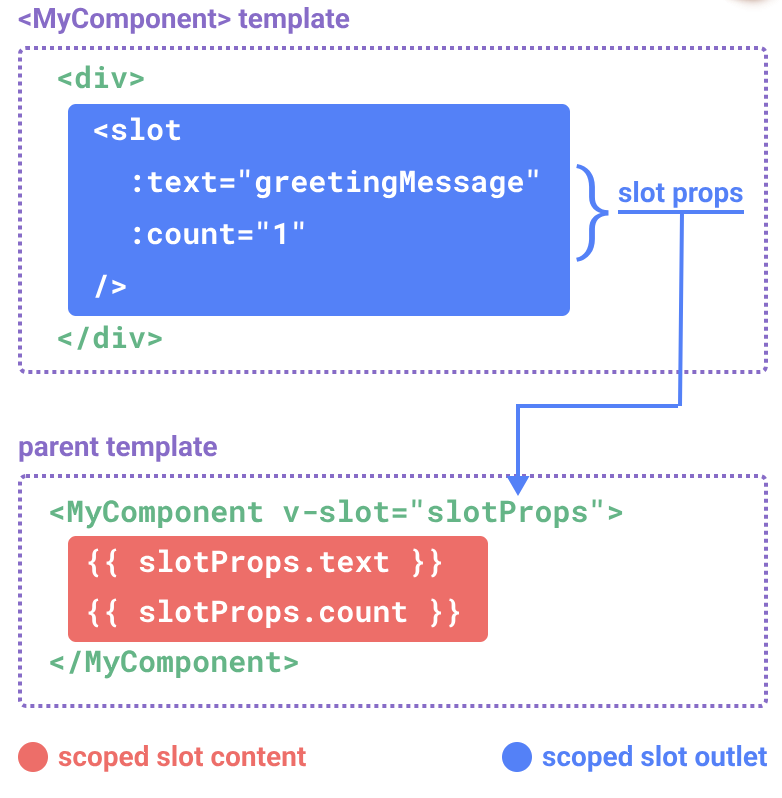
\includegraphics{./img/scoped-slots.1c6d5876.png} 
\end{center}
    


\columnratio{0.55}
\begin{paracol}{2}
 
\switchcolumn[0]*%%%%%%%
\href{https://play.vuejs.org/\#eNp9kMEKgzAMhl8l9OJlU3aVOhg7C3uAXsRlTtC2tFE2pO++dA5xMnZqk+b/8/2dxMnadBxQ5EL62rWWwCMN9qh021vjCMrn2fBNoya4OdNDkmarXhQnSstsVrOOC8LedhVhrEiuHca97wwVSsTj4oz1SvAUgKJpgqWZEj4IQoCvZm0Gtgghzss1BDvIbFkqdmID+CNdbbQnaBwitbop0fuqQSgguWPXmX+JePe1HT/QMtJBHnE51MZOCcjfzPx04JxsydPzp2Szxxo7vABY1I/p}{Try
it in the Playground}
\switchcolumn
\href{https://play.vuejs.org/\#eNp9kMEKgzAMhl8l9OJlU3aVOhg7C3uAXsRlTtC2tFE2pO++dA5xMnZqk+b/8/2dxMnadBxQ5EL62rWWwCMN9qh021vjCMrn2fBNoya4OdNDkmarXhQnSstsVrOOC8LedhVhrEiuHca97wwVSsTj4oz1SvAUgKJpgqWZEj4IQoCvZm0Gtgghzss1BDvIbFkqdmID+CNdbbQnaBwitbop0fuqQSgguWPXmX+JePe1HT/QMtJBHnE51MZOCcjfzPx04JxsydPzp2Szxxo7vABY1I/p}{在演练场中尝试一下}
\switchcolumn[0]*%%%%%%%
The props passed to the slot by the child are available as the value of
the corresponding \texttt{v-slot} directive, which can be accessed by
expressions inside the slot.
\switchcolumn
子组件传入插槽的 props 作为了 \texttt{v-slot}
指令的值,可以在插槽内的表达式中访问。
\switchcolumn[0]*%%%%%%%
You can think of a scoped slot as a function being passed into the child
component. The child component then calls it, passing props as
arguments:
\switchcolumn
你可以将作用域插槽类比为一个传入子组件的函数。子组件会将相应的 props
作为参数传给它:
\switchcolumn[0]*%%%%%%%
\begin{codeJs}
MyComponent({
  // 类比默认插槽,将其想成一个函数
  default: (slotProps) => {
    return `${slotProps.text} ${slotProps.count}`
  }
})
function MyComponent(slots) {
  const greetingMessage = 'hello'
  return `<div>${
    // 在插槽函数调用时传入 props
    slots.default({ text: greetingMessage, count: 1 })
  }</div>`
}
\end{codeJs}
\switchcolumn
\begin{codeJs}
MyComponent({
  // 类比默认插槽,将其想成一个函数
  default: (slotProps) => {
    return `${slotProps.text} ${slotProps.count}`
  }
})
function MyComponent(slots) {
  const greetingMessage = 'hello'
  return `<div>${
    // 在插槽函数调用时传入 props
    slots.default({ text: greetingMessage, count: 1 })
  }</div>`
}
\end{codeJs}
\switchcolumn[0]*%%%%%%%
In fact, this is very close to how scoped slots are compiled, and how
you would use scoped slots in manual
\href{https://vuejs.org/guide/extras/render-function.html}{render
functions}.
\switchcolumn
实际上,这已经和作用域插槽的最终代码编译结果、以及手动编写\href{https://cn.vuejs.org/guide/extras/render-function.html}{渲染函数}时使用作用域插槽的方式非常类似了。
\switchcolumn[0]*%%%%%%%
Notice how \texttt{v-slot="slotProps"} matches the slot function
signature. Just like with function arguments, we can use destructuring
in \texttt{v-slot}:
\switchcolumn
\texttt{v-slot="slotProps"}
可以类比这里的函数签名,和函数的参数类似,我们也可以在 \texttt{v-slot}
中使用解构:
\switchcolumn[0]*%%%%%%%
\begin{codeHtml}
<MyComponent v-slot="{ text, count }">
  {{ text }} {{ count }}
</MyComponent>
\end{codeHtml}
\switchcolumn
\begin{codeHtml}
<MyComponent v-slot="{ text, count }">
  {{ text }} {{ count }}
</MyComponent>
\end{codeHtml} 
\end{paracol}

\columnratio{0.55}
\begin{paracol}{2}
 
\switchcolumn[0]*%%%%%%%
\subsubsection{Named Scoped Slots}
\switchcolumn
\subsubsection{具名作用域插槽}
\switchcolumn[0]*%%%%%%%
Named scoped slots work similarly - slot props are accessible as the
value of the \texttt{v-slot} directive:
\texttt{v-slot:name="slotProps"}. When using the shorthand, it looks
like this:
\switchcolumn
具名作用域插槽的工作方式也是类似的,插槽 props 可以作为 \texttt{v-slot}
指令的值被访问到:\texttt{v-slot:name="slotProps"}。当使用缩写时是这样:
\switchcolumn[0]*%%%%%%%
\begin{codeHtml}
<MyComponent>
  <template #header="headerProps">
    {{ headerProps }}
  </template>
  <template #default="defaultProps">
    {{ defaultProps }}
  </template>
  <template #footer="footerProps">
    {{ footerProps }}
  </template>
</MyComponent>
\end{codeHtml}
\switchcolumn
\begin{codeHtml}
<MyComponent>
  <template #header="headerProps">
    {{ headerProps }}
  </template>
  <template #default="defaultProps">
    {{ defaultProps }}
  </template>
  <template #footer="footerProps">
    {{ footerProps }}
  </template>
</MyComponent>
\end{codeHtml}
\switchcolumn[0]*%%%%%%%
Passing props to a named slot:
\switchcolumn
向具名插槽中传入 props:
\switchcolumn[0]*%%%%%%%
\begin{codeHtml}
<slot name="header" message="hello"></slot>
\end{codeHtml}
\switchcolumn
\begin{codeHtml}
<slot name="header" message="hello"></slot>
\end{codeHtml}
\switchcolumn[0]*%%%%%%%
Note the \texttt{name} of a slot won't be included in the props because
it is reserved - so the resulting \texttt{headerProps} would be
\texttt{\{\ message:\ \textquotesingle{}hello\textquotesingle{}\ \}}.
\switchcolumn
注意插槽上的 \texttt{name} 是一个 Vue 特别保留的 attribute,不会作为
props 传递给插槽。因此最终 \texttt{headerProps} 的结果是
\texttt{\{\ message:\ \textquotesingle{}hello\textquotesingle{}\ \}}。
\switchcolumn[0]*%%%%%%%
If you are mixing named slots with the default scoped slot, you need to
use an explicit \texttt{\textless{}template\textgreater{}} tag for the
default slot. Attempting to place the \texttt{v-slot} directive directly
on the component will result in a compilation error. This is to avoid
any ambiguity about the scope of the props of the default slot. For
example:
\switchcolumn
如果你同时使用了具名插槽与默认插槽,则需要为默认插槽使用显式的
\texttt{\textless{}template\textgreater{}} 标签。尝试直接为组件添加
\texttt{v-slot} 指令将导致编译错误。这是为了避免因默认插槽的 props
的作用域而困惑。举例:
\switchcolumn[0]*%%%%%%%
\begin{codeHtml}
<!-- 该模板无法编译 -->
<template>
  <MyComponent v-slot="{ message }">
    <p>{{ message }}</p>
    <template #footer>
      <!-- message 属于默认插槽,此处不可用 -->
      <p>{{ message }}</p>
    </template>
  </MyComponent>
</template>
\end{codeHtml}
\switchcolumn
\begin{codeHtml}
<!-- 该模板无法编译 -->
<template>
  <MyComponent v-slot="{ message }">
    <p>{{ message }}</p>
    <template #footer>
      <!-- message 属于默认插槽,此处不可用 -->
      <p>{{ message }}</p>
    </template>
  </MyComponent>
</template>
\end{codeHtml}
\switchcolumn[0]*%%%%%%%
Using an explicit \texttt{\textless{}template\textgreater{}} tag for the
default slot helps to make it clear that the \texttt{message} prop is
not available inside the other slot:
\switchcolumn
为默认插槽使用显式的 \texttt{\textless{}template\textgreater{}}
标签有助于更清晰地指出 \texttt{message} 属性在其他插槽中不可用:
\switchcolumn[0]*%%%%%%%
\begin{codeHtml}
<template>
  <MyComponent>
    <!-- 使用显式的默认插槽 -->
    <template #default="{ message }">
      <p>{{ message }}</p>
    </template>
    <template #footer>
      <p>Here's some contact info</p>
    </template>
  </MyComponent>
</template>
\end{codeHtml}
\switchcolumn
\begin{codeHtml}
<template>
  <MyComponent>
    <!-- 使用显式的默认插槽 -->
    <template #default="{ message }">
      <p>{{ message }}</p>
    </template>
    <template #footer>
      <p>Here's some contact info</p>
    </template>
  </MyComponent>
</template>
\end{codeHtml}
\end{paracol}

\columnratio{0.55}
\begin{paracol}{2}
  
\switchcolumn[0]*%%%%%%%
\subsubsection{Fancy List Example}
\switchcolumn
\subsubsection{高级列表组件示例}
\switchcolumn[0]*%%%%%%%
You may be wondering what would be a good use case for scoped slots.
Here's an example: imagine a \texttt{\textless{}FancyList\textgreater{}}
component that renders a list of items - it may encapsulate the logic
for loading remote data, using the data to display a list, or even
advanced features like pagination or infinite scrolling. However, we
want it to be flexible with how each item looks and leave the styling of
each item to the parent component consuming it. So the desired usage may
look like this:
\switchcolumn
你可能想问什么样的场景才适合用到作用域插槽,这里我们来看一个
\texttt{\textless{}FancyList\textgreater{}}
组件的例子。它会渲染一个列表,并同时会封装一些加载远端数据的逻辑、使用数据进行列表渲染、或者是像分页或无限滚动这样更进阶的功能。然而我们希望它能够保留足够的灵活性,将对单个列表元素内容和样式的控制权留给使用它的父组件。我们期望的用法可能是这样的:
\switchcolumn[0]*%%%%%%%
\begin{codeHtml}
<FancyList :api-url="url" :per-page="10">
  <template #item="{ body, username, likes }">
    <div class="item">
      <p>{{ body }}</p>
      <p>by {{ username }} | {{ likes }} likes</p>
    </div>
  </template>
</FancyList>
\end{codeHtml}
\switchcolumn
\begin{codeHtml}
<FancyList :api-url="url" :per-page="10">
  <template #item="{ body, username, likes }">
    <div class="item">
      <p>{{ body }}</p>
      <p>by {{ username }} | {{ likes }} likes</p>
    </div>
  </template>
</FancyList>
\end{codeHtml}
\switchcolumn[0]*%%%%%%%
Inside \texttt{\textless{}FancyList\textgreater{}}, we can render the
same \texttt{\textless{}slot\textgreater{}} multiple times with
different item data (notice we are using \texttt{v-bind} to pass an
object as slot props):
\switchcolumn
在 \texttt{\textless{}FancyList\textgreater{}} 之中,我们可以多次渲染
\texttt{\textless{}slot\textgreater{}} 并每次都提供不同的数据
(注意我们这里使用了 \texttt{v-bind} 来传递插槽的 props):
\switchcolumn[0]*%%%%%%%
\begin{codeHtml}
<ul>
  <li v-for="item in items">
    <slot name="item" v-bind="item"></slot>
  </li>
</ul>
\end{codeHtml}
\switchcolumn
\begin{codeHtml}
<ul>
  <li v-for="item in items">
    <slot name="item" v-bind="item"></slot>
  </li>
</ul>
\end{codeHtml}
\switchcolumn[0]*%%%%%%%
\href{https://play.vuejs.org/\#eNqFU2Fv0zAQ/StHJtROapNuZTBCNwnQQKBpTGxCQss+uMml8+bYlu2UlZL/zjlp0lQa40sU3/nd3Xv3vA7eax0uSwziYGZTw7UDi67Up4nkhVbGwScm09U5tw5yowoYhFEX8cBBImdRgyQMHRwWWjCHdAKYbdFM83FpxEkS0DcJINZoxpotkCIHkySo7xOixcMep19KrmGustUISotGsgJHIPgDWqg6DKEyvoRUMGsJ4HG9HGX16bqpAlU1izy5baqDFegYweYroMttMwLAHx/Y9Kyan36RWUTN2+mjXfpbrei8k6SjdSuBYFOlMaNI6AeAtcflSrqx5b8xhkl4jMU7H0yVUCaGvVeH8+PjKYWqWnpf5DQYBTtb+fc612Awh2qzzGaBiUyVpBVpo7SFE8gw5xIv/Wl4M9gsbjCCQbuywe3+FuXl9iiqO7xpElEEhUofKFQo2mTGiFiOLr3jcpFImuiaF6hKNxzuw8lpw7kuEy6ZKJGK3TR6NluLYXBVqwRXQjkLn0ueIc3TLonyZ0sm4acqKVovKIbDCVQjGsb1qvyg2telU4Yzz6eHv6ARBWdwjVqUNCbbFjqgQn6aW1J8RKfJhDg+5/lStG4QHJZjnpO5XjT0BMqFu+uZ81yxjEQJw7A1kOA76FyZjaWBy0akvu8tCQKeQ+d7wsy5zLpz1FlzU3kW1QP+x40ApWgWAySEJTv6/NitNMkllcTakwCaZZ5ADEf6cROas/RhYVQps5igEpkZLwzRROmG04OjDBcj7+Js+vYQDo9e0uH1qzeY5/s1vtaaqG969+vTTrsmBTMLLv12nuy7l+d5W673SBzxkzlfhPdWSXokdZMkSFWhuUDzTTtOnk6CuG2fBEwI9etrHXOmRLJUE0/vMH14In5vH30sCS4Nkr+WmARdztHQ6Jr02dUFPtJ/lyxUVgq6/UzyO1olSj9jc+0DcaWxe/fqab/UT51Uu7Znjw6lbUn5QWtR6vtJQM//4zPUt+NOw+lGzCqo/gLm1QS8}{Try
it in the Playground}
\switchcolumn
\href{https://play.vuejs.org/\#eNqFU2Fv0zAQ/StHJtROapNuZTBCNwnQQKBpTGxCQss+uMml8+bYlu2UlZL/zjlp0lQa40sU3/nd3Xv3vA7eax0uSwziYGZTw7UDi67Up4nkhVbGwScm09U5tw5yowoYhFEX8cBBImdRgyQMHRwWWjCHdAKYbdFM83FpxEkS0DcJINZoxpotkCIHkySo7xOixcMep19KrmGustUISotGsgJHIPgDWqg6DKEyvoRUMGsJ4HG9HGX16bqpAlU1izy5baqDFegYweYroMttMwLAHx/Y9Kyan36RWUTN2+mjXfpbrei8k6SjdSuBYFOlMaNI6AeAtcflSrqx5b8xhkl4jMU7H0yVUCaGvVeH8+PjKYWqWnpf5DQYBTtb+fc612Awh2qzzGaBiUyVpBVpo7SFE8gw5xIv/Wl4M9gsbjCCQbuywe3+FuXl9iiqO7xpElEEhUofKFQo2mTGiFiOLr3jcpFImuiaF6hKNxzuw8lpw7kuEy6ZKJGK3TR6NluLYXBVqwRXQjkLn0ueIc3TLonyZ0sm4acqKVovKIbDCVQjGsb1qvyg2telU4Yzz6eHv6ARBWdwjVqUNCbbFjqgQn6aW1J8RKfJhDg+5/lStG4QHJZjnpO5XjT0BMqFu+uZ81yxjEQJw7A1kOA76FyZjaWBy0akvu8tCQKeQ+d7wsy5zLpz1FlzU3kW1QP+x40ApWgWAySEJTv6/NitNMkllcTakwCaZZ5ADEf6cROas/RhYVQps5igEpkZLwzRROmG04OjDBcj7+Js+vYQDo9e0uH1qzeY5/s1vtaaqG969+vTTrsmBTMLLv12nuy7l+d5W673SBzxkzlfhPdWSXokdZMkSFWhuUDzTTtOnk6CuG2fBEwI9etrHXOmRLJUE0/vMH14In5vH30sCS4Nkr+WmARdztHQ6Jr02dUFPtJ/lyxUVgq6/UzyO1olSj9jc+0DcaWxe/fqab/UT51Uu7Znjw6lbUn5QWtR6vtJQM//4zPUt+NOw+lGzCqo/gLm1QS8}{在演练场中尝试一下}
\end{paracol}


\columnratio{0.55}
\begin{paracol}{2}
 
\switchcolumn[0]*%%%%%%%
\subsubsection{Renderless Components}
\switchcolumn
\subsubsection{无渲染组件}
\switchcolumn[0]*%%%%%%%
The \texttt{\textless{}FancyList\textgreater{}} use case we discussed
above encapsulates both reusable logic (data fetching, pagination etc.)
and visual output, while delegating part of the visual output to the
consumer component via scoped slots.
\switchcolumn
上面的 \texttt{\textless{}FancyList\textgreater{}}
案例同时封装了可重用的逻辑 (数据获取、分页等)
和视图输出,但也将部分视图输出通过作用域插槽交给了消费者组件来管理。
\switchcolumn[0]*%%%%%%%
If we push this concept a bit further, we can come up with components
that only encapsulate logic and do not render anything by themselves -
visual output is fully delegated to the consumer component with scoped
slots. We call this type of component a \textbf{Renderless Component}.
\switchcolumn
如果我们将这个概念拓展一下,可以想象的是,一些组件可能只包括了逻辑而不需要自己渲染内容,视图输出通过作用域插槽全权交给了消费者组件。我们将这种类型的组件称为\textbf{无渲染组件}。
\switchcolumn[0]*%%%%%%%
An example renderless component could be one that encapsulates the logic
of tracking the current mouse position:
\switchcolumn
这里有一个无渲染组件的例子,一个封装了追踪当前鼠标位置逻辑的组件:
\switchcolumn[0]*%%%%%%%
\begin{codeHtml}
<MouseTracker v-slot="{ x, y }">
  Mouse is at: {{ x }}, {{ y }}
</MouseTracker>
\end{codeHtml}
\switchcolumn
\begin{codeHtml}
<MouseTracker v-slot="{ x, y }">
  Mouse is at: {{ x }}, {{ y }}
</MouseTracker>
\end{codeHtml}
\switchcolumn[0]*%%%%%%%
\href{https://play.vuejs.org/\#eNqNUcFqhDAQ/ZUhF12w2rO4Cz301t5aaCEX0dki1SQko6uI/96J7i4qLPQQmHmZ9+Y9ZhQvxsRdiyIVmStsZQgcUmtOUlWN0ZbgXbcOP2xe/KKFs9UNBHGyBj09kCpLFj4zuSFsTJ0T+o6yjUb35GpNRylG6CMYYJKCpwAkzWNQOcgphZG/YZoiX/DQNAttFjMrS+6LRCT2rh6HGsHiOQKtmKIIS19+qmZpYLrmXIKxM1Vo5Yj9HD0vfD7ckGGF3LDWlOyHP/idYPQCfdzldTtjscl/8MuDww78lsqHVHdTYXjwCpdKlfoS52X52qGit8oRKrRhwHYdNrrDILouPbCNVZCtgJ1n/6Xx8JYAmT8epD3fr5cC0oGLQYpkd4zpD27R0vA=}{Try
it in the Playground}
\switchcolumn
\href{https://play.vuejs.org/\#eNqNUcFqhDAQ/ZUhF12w2rO4Cz301t5aaCEX0dki1SQko6uI/96J7i4qLPQQmHmZ9+Y9ZhQvxsRdiyIVmStsZQgcUmtOUlWN0ZbgXbcOP2xe/KKFs9UNBHGyBj09kCpLFj4zuSFsTJ0T+o6yjUb35GpNRylG6CMYYJKCpwAkzWNQOcgphZG/YZoiX/DQNAttFjMrS+6LRCT2rh6HGsHiOQKtmKIIS19+qmZpYLrmXIKxM1Vo5Yj9HD0vfD7ckGGF3LDWlOyHP/idYPQCfdzldTtjscl/8MuDww78lsqHVHdTYXjwCpdKlfoS52X52qGit8oRKrRhwHYdNrrDILouPbCNVZCtgJ1n/6Xx8JYAmT8epD3fr5cC0oGLQYpkd4zpD27R0vA=}{在演练场中尝试一下}
\switchcolumn[0]*%%%%%%%
While an interesting pattern, most of what can be achieved with
Renderless Components can be achieved in a more efficient fashion with
Composition API, without incurring the overhead of extra component
nesting. Later, we will see how we can implement the same mouse tracking
functionality as a
\href{https://vuejs.org/guide/reusability/composables.html}{Composable}.
\switchcolumn
虽然这个模式很有趣,但大部分能用无渲染组件实现的功能都可以通过组合式 API
以另一种更高效的方式实现,并且还不会带来额外组件嵌套的开销。之后我们会在\href{https://cn.vuejs.org/guide/reusability/composables.html}{组合式函数}一章中介绍如何更高效地实现追踪鼠标位置的功能。
\switchcolumn[0]*%%%%%%%
That said, scoped slots are still useful in cases where we need to both
encapsulate logic \textbf{and} compose visual output, like in the
\texttt{\textless{}FancyList\textgreater{}} example.
\switchcolumn
尽管如此,作用域插槽在需要\textbf{同时}封装逻辑、组合视图界面时还是很有用,就像上面的
\texttt{\textless{}FancyList\textgreater{}} 组件那样。
\end{paracol}



\columnratio{0.55}
\begin{paracol}{2}
 
\end{paracol}
